%%%%% --------------------------------------------------------------------------------
%%
%%                               Document Template
%%
%%%%% --------------------------------------------------------------------------------
%% Copyright (C) Huangrui Mo <huangrui.mo@gmail.com> 
%% This is free software: you can redistribute it and/or modify it
%% under the terms of the GNU General Public License as published by
%% the Free Software Foundation, either version 3 of the License, or
%% (at your option) any later version.
%%%%% --------------------------------------------------------------------------------
%%
%%%%************************ Document Class Declaration ******************************
%%
\documentclass[doublesided]{Style/ucasthesis}% thesis template of UCAS
%% Multiple optional arguments:
%% [scheme = plain] % for thesis writing of international students
%% [<singlesided|doublesided|printcopy>] % single-sided, double-sided, or print layout
%% [draftversion] % show draft version information, default is no show
%% [fontset = <adobe|...>] % specify font set, default is automatic detection
%% [standard options for ctex class]
%%%%% --------------------------------------------------------------------------------
%%
%%%%************************* Command Define and Settings ****************************
%%
\usepackage[myhdr]{Style/commons}% common settings
%% usage: \usepackage[option1,option2,...,optionN]{commons}
%% Multiple optional arguments:
%% [<numbered|authoryear|alpha>] % citation and reference style
%% <numbered>: textual: Jones [1]; parenthetical: [1]. default style
%% <authoryear>: textual: Jones (1995); parenthetical: (Jones, 1995)
%% <alpha>: textual: not available; parenthetical: [Jon95]
%% [myhdr] % one available header and footer style, will enable fancyhdr
%% [lscape] % provide landscape layout environment
%% [geometry] % configure page layout by geometry package
%% [list] % enable enhanced list environments, useful for Algorithm and Coding
%% [color] % enable color package to use color, default package is xcolor
%% [background] % enable page background, will auto enable color package
%% [tikz] % enable tikz for complex diagrams, will auto enbale color package
%% [table] % enable a table package for complex tables, default is ctable
%% [math] % enable some extra math packages
\usepackage{Style/custom}% user defined commands
\usepackage{setspace}
%%%%% --------------------------------------------------------------------------------
%%
%%%%******************************** Content *****************************************
%%
\begin{document}
%%
%%%%% --------------------------------------------------------------------------------
%%
%%%%******************************** Frontmatter *************************************
%%
%% Frontmatter of Title page, Table of contents, Preface chapter.
\frontmatter
%%
%% >>> Frontpages
%%
%---------------------------------------------------------------------------%
%->> Titlepage information
%---------------------------------------------------------------------------%
%-
%-> Chinese titlepage
%-
\confidential{}% confidential level
\schoollogo{scale=0.112}{ucas_logo}% university logo
\title{中国科学院大学学位论文\LaTeX{}模板 {$~^{\pi}\pi^{\pi}$}}% \title[short title for headers]{Long title of thesis}
\author{肖攀}% name of author
\advisor{方广有~研究员}% supervisor
\advisorsec{中国科学院电子学研究所}% co-supervisor
\degree{博士}% degree
\degreetype{工学}% degree type
\major{电磁场与微波技术}% major
\institute{中国科学院电子学研究所}% institute of author
%\chinesedate{2014~年~6~月}% customized date, 6 for summer and 12 for winter graduation
%-
%-> English titlepage
%-
\englishtitle{\LaTeX{} Thesis Template\\ of \\ The University of Chinese Academy of Sciences {$~^{\pi}\pi^{\pi}$}}
\englishauthor{Pan Xiao}
\englishadvisor{Professor Guangyou Fang}
\englishdegree{Doctor}% degree type <Doctor|Master> of <Philosophy|Natural Science|Engineering>
\englishthesistype{Dissertation}% thesis type <thesis|dissertation>
\englishmajor{Engineering}% major
\englishinstitute{Institute of Electronics, Chinese Academy of Sciences}
%\englishdate{June, 2014}% customized date
%-
%-> Create titlepages
%-
\maketitle
\makeenglishtitle
%-
%-> Author's declaration
%-
\makedeclaration
%-
%-> Chinese abstract
%-
\chapter{摘\quad 要}
\setcounter{page}{1}% set page number
\pagenumbering{Roman}% set large roman

本文是中国科学院大学学位论文模板ucasthesis的使用说明文档。主要内容为介绍\LaTeX{}文档类ucasthesis的用法,以及如何使用\LaTeX{}快速高效地撰写学位论文。

\keywords{中国科学院大学,学位论文,\LaTeX{}模板}
%-
%-> English abstract
%-
\chapter{Abstract}

This paper is a help documentation for the \LaTeX{} class ucasthesis, which is  a thesis template for the University of Chinese Academy of Sciences. The main content is about how to use the ucasthesis, as well as how to write thesis efficiently by using \LaTeX{}.

\englishkeywords{University of Chinese Academy of Sciences (UCAS), Thesis, \LaTeX{} Template}
%---------------------------------------------------------------------------%

%%
%%% >>> List of Content
%%
\intotoc{\contentsname}% add a corresponding item to the contents table and bookmark
\tableofcontents% contents catalog
\intotoc{\listfigurename}% add a corresponding item to the contents table and bookmark
\listoffigures% figures catalog
\intotoc{\listtablename}% add a corresponding item to the contents table and bookmark
\listoftables% tables catalog
%%
%% >>> prematter
%%
\chapter*{符号列表}
\chaptermark{符号列表}

\section*{字符}
\nomenclatureitem[\textbf{Unit}]{\textbf{Symbol}}{\textbf{Description}}
\nomenclatureitem[$\Unit{m^{2} \cdot s^{-2} \cdot K^{-1}}$]{$R$}{the gas constant}
\nomenclatureitem[$\Unit{m^{2} \cdot s^{-2} \cdot K^{-1}}$]{$C_v$}{specific heat capacity at constant volume}
\nomenclatureitem[$\Unit{m^{2} \cdot s^{-2} \cdot K^{-1}}$]{$C_p$}{specific heat capacity at constant pressure}
\nomenclatureitem[$\Unit{m^{2} \cdot s^{-2}}$]{$E$}{specific total energy}
\nomenclatureitem[$\Unit{m^{2} \cdot s^{-2}}$]{$e$}{specific internal energy}
\nomenclatureitem[$\Unit{m^{2} \cdot s^{-2}}$]{$h_T$}{specific total enthalpy}
\nomenclatureitem[$\Unit{m^{2} \cdot s^{-2}}$]{$h$}{specific enthalpy}
\nomenclatureitem[$\Unit{kg \cdot m \cdot s^{-3} \cdot K^{-1}}$]{$k$}{thermal conductivity}
\nomenclatureitem[$\Unit{kg \cdot m^{-1} \cdot s^{-2}}$]{$S_{ij}$}{deviatoric stress tensor}
\nomenclatureitem[$\Unit{kg \cdot m^{-1} \cdot s^{-2}}$]{$\tau_{ij}$}{viscous stress tensor}
\nomenclatureitem[$\Unit{1}$]{$\delta_{ij}$}{Kronecker tensor}
\nomenclatureitem[$\Unit{1}$]{$I_{ij}$}{identity tensor}

\section*{算子}
\nomenclatureitem{\textbf{Symbol}}{\textbf{Description}}
\nomenclatureitem{$\Delta$}{difference}
\nomenclatureitem{$\nabla$}{gradient operator}
\nomenclatureitem{$\delta^{\pm}$}{upwind-biased interpolation scheme}

\section*{缩写}
\nomenclatureitem{CFD}{Computational Fluid Dynamics}
\nomenclatureitem{CFL}{Courant-Friedrichs-Lewy}
\nomenclatureitem{EOS}{Equation of State}
\nomenclatureitem{JWL}{Jones-Wilkins-Lee}
\nomenclatureitem{WENO}{Weighted Essentially Non-oscillatory}
\nomenclatureitem{ZND}{Zel'dovich-von Neumann-Doering}

% list of symbols, preface of books
%%
%%%%% --------------------------------------------------------------------------------
%%
%%%%******************************** Mainmatter **************************************
%%
%% Main topics.
\mainmatter
%%
%%% >>> Main Contents
%%
% !TeX encoding = UTF-8
% !TeX program = pdfLaTeX
% !TeX root = ../Thesis.tex
% !TeX spellcheck = None

%%%%% --------------------------------------------------------------------------------
%%
%%%%******************************* Main Content *************************************
%%
%%% ++++++++++++++++++++++++++++++++++++++++++++++++++++++++++++++++++++++++++++++++++

\chapter{引言}
\label{chap:introduction}

考虑到大多数用户并无\LaTeX{}使用经验,本模板将\LaTeX{}的复杂性尽可能地进行了封装,开放出简单的接口,以便于使用者可以轻易地使用。同时,对使用\LaTeX{}撰写论文所遇到的一些主要难题,如插入图片、文献索引等,进行了详细的说明,并提供了相应的代码样本,理解了上述问题后,对于初学者而言,使用此模板撰写其学文论文将不存在实质性的困难。所以,如果您是初学者,请不要直接放弃,因为同样作为初学者的我,十分明白让\LaTeX{}变得简单易用的重要性,而这正是本模板所体现的。

此中国科学院大学学位论文模板ucasthesis基于中科院数学与系统科学研究院吴凌云研究员的CASthesis模板发展而来。当前ucasthesis 模板满足最新的中国科学院大学学位论文撰写要求和封面设定。模板兼顾不同操作系统 (Windows,Linux,Mac OS) 和\LaTeX{}编译引擎(pdflatex,xelatex,lualatex),完美地支持中文书签、中文渲染、中文粗体显示、拷贝PDF中的文本到其他文本编辑器等特性,此外,对模板的文档结构进行了精心设计,撰写了编译脚本提高模板的易用性和使用效率。

宏包的目的是简化学位论文的撰写,模板文档的默认设定是十分规范的,从而论文作者可以将精力集中到论文的内容上,而不需要在版面设置上花费精力。 同时,在编写模板的\LaTeX{}文档代码过程中,作者对各结构和命令进行了十分详细的注解,并提供了整洁一致的代码结构,对文档的仔细阅读可以为初学的您提供一个学习\LaTeX{}的窗口。除此之外,整个模板的架构十分注重通用性,事实上,本模板不仅是中国科学院大学学文论文模板,同时,也是使用\LaTeX{}撰写中英文Article或Book的通用模板,并为使用者的个性化设定提供了接口和相应的代码。

\section{系统要求}\label{sec:system}

\href{https://github.com/mohuangrui/ucasthesis}{\texttt{ucasthesis}} 宏包可以在目前主流的 \href{https://en.wikibooks.org/wiki/LaTeX/Introduction}{\LaTeX{}} 编译系统中使用,例如C\TeX{}套装 (请勿混淆C\TeX{}套装与ctex宏包。C\TeX{}套装是集成了许多\LaTeX{}组件的\LaTeX{}编译系统,因已停止维护,\textbf{不再建议使用}。 \href{https://ctan.org/pkg/ctex?lang=en}{ctex} 宏包就如同ucasthesis一样,是\LaTeX{}命令集,其维护状态非常活跃,并被所有主流的\LaTeX{}编译系统所默认集成,是几乎所有\LaTeX{}中文文档的核心架构。)、MiK\TeX{}、\TeX{}Live。推荐的 \href{https://en.wikibooks.org/wiki/LaTeX/Installation}{\LaTeX{}编译系统} 和 \href{https://en.wikibooks.org/wiki/LaTeX/Installation}{\LaTeX{}文本编辑器} 为
\begin{center}
    %\footnotesize% fontsize
    %\setlength{\tabcolsep}{4pt}% column separation
    %\renewcommand{\arraystretch}{1.5}% row space 
    \begin{tabular}{lcc}
        \hline\hline
        %\multicolumn{num_of_cols_to_merge}{alignment}{contents} \\
        %\cline{i-j}% partial hline from column i to column j
        操作系统 & \LaTeX{}编译系统 & \LaTeX{}文本编辑器\\
        \hline
        Linux & \href{https://www.tug.org/texlive/acquire-netinstall.html}{\TeX{}Live Full} & \href{http://www.xm1math.net/texmaker/}{Texmaker}\\
        MacOS & \href{https://www.tug.org/mactex/}{Mac\TeX{} Full} & \href{http://www.xm1math.net/texmaker/}{Texmaker}\\
        Windows & \href{https://www.tug.org/texlive/acquire-netinstall.html}{\TeX{}Live Full} 或 \href{https://miktex.org/download}{Mik\TeX{}} & \href{http://www.xm1math.net/texmaker/}{Texmaker}\\
        \hline\hline
    \end{tabular}
\end{center}

\LaTeX{}编译系统 (如MiK\TeX{}、\TeX{}Live) 用于提供编译环境,\LaTeX{}文本编辑器 (如Texmaker) 用于编辑\TeX{}源文件。请一定从上述各软件的官网下载安装程序,勿使用其它程序源。\textbf{\LaTeX{}编译系统和\LaTeX{}编辑器分别安装成功后,用户即完成了\LaTeX{}的系统配置},无需其他手动干预和配置。若用户的系统原带有旧版的\LaTeX{}编译系统并想安装新版,其\textbf{先卸载干净旧版再安装新版}。

\section{问题反馈}

非针对模板本身的问题,而是关于\LaTeX{}的知识性问题,请自行查阅资料,特别是 \href{https://en.wikibooks.org/wiki/LaTeX}{\LaTeX{} Wikibook}。

若遇到关于模板编译和样式设计的问题,请\textbf{先仔细阅读此说明文档,特别是“常见问题”(章节~\ref{sec:qa})}。若问题仍无法得到解决,请\textbf{先将问题理解清楚并描述清楚,再将问题反馈}至 \href{https://github.com/mohuangrui/ucasthesis/issues}{Github/ucasthesis/issues}。有效地反馈问题,为大家都省时间。

欢迎大家有效地反馈模板不足之处,一起不断改进模板。希望大家向同事积极推广\LaTeX{},一起更高效地做科研。

\section{模板下载}

\begin{center}
    \href{https://github.com/mohuangrui/ucasthesis}{Github/ucasthesis}: \url{https://github.com/mohuangrui/ucasthesis}
\end{center}


\chapter{使用简介}
\label{chap:guide}

为方便使用及更好地展示\LaTeX{}排版的优秀特性,本人对模板的框架和文件体系进行了细致地处理,尽可能地对各个功能和板块进行了模块化和封装,对于初学者来说,众多的文件目录也许会让人觉得有些无所适从,但阅读完下面的使用说明后,您会发现原来使用思路是简单而清晰的,而且,当对\LaTeX{}有一定的认识和了解后,会发现其相对Word类排版系统的极具吸引力的优秀特性。所以,如果您是初学者,请不要退缩,请稍加尝试和坚持,让自己领略到\LaTeX{}的非凡魅力,并可以通过阅读相关资料如Wikibook\citep{wikibook2014latex}来完善自己的使用知识。

\section{先试试效果}

\begin{enumerate}
    \item 安装软件:根据所用操作系统和章节~\ref{sec:system}中的信息安装\LaTeX{}编译环境。
    \item 获取模板:下载 \href{https://github.com/mohuangrui/ucasthesis}{ucasthesis} 模板并解压。ucasthesis模板不仅提供了相应的类文件,同时也提供了包括参考文献等在内的完成学位论文的一切要素,所以,下载时,推荐下载整个ucasthesis文件夹,而不是单独的文档类。
    \item 编译模板:
        \begin{enumerate}
            \item Windows用户:双击运行artratex.bat脚本。
            \item Linux或Mac OS用户: \verb|terminal| -> \verb|chmod +x ./artratex.sh| -> \verb|./artratex.sh xa|
            \item 任意系统:都可使用\LaTeX{}编辑器打开Thesis.tex文件进行编译。
        \end{enumerate}
    \item 处理错误:若编译中遇到了问题,请先查看“常见问题”(章节~\ref{sec:qa})。
\end{enumerate}

编译完成后,即可获得本PDF说明文档。而这也完成了学习使用此模板撰写论文的一半进程。什么?这就学成一半了,这么简单???,是的,就这么简单!

\section{文档目录简介}

\subsection{Thesis.tex}

Thesis.tex为主文档,其设计和规划了论文的整体框架,通过对其的阅读可以让用户了解整个论文框架的搭建。

\subsection{编译脚本}

\begin{itemize}
    \item Windows用户:双击Dos脚本artratex.bat可得全编译后的PDF文档。
    \item Linux或Mac OS用户:在terminal中运行
        \begin{itemize}
            \item \verb|./artratex.sh xa|:获得全编译后的PDF文档
            \item \verb|./artratex.sh x|:快速编译模式
        \end{itemize}
    \item 全编译指运行 \verb|latex引擎+bibtex+latex引擎+latex引擎| 以正确生成所有的引用链接,如目录,参考文献及引用等。在写作过程中若无添加新的引用,则可用快速编译,即只运行一遍\LaTeX{}编译引擎以减少编译时间。
\end{itemize}

\subsection{Tmp文件夹}

运行编译脚本后,编译所生成的文档皆存于Tmp文件夹内,包括编译得到的PDF文档,其存在是为了保持工作空间的整洁,因为好的心情是很重要的。

\subsection{Style文件夹}

Style文件夹内包含ucasthesis文档类的定义文件和配置文件,对于有特殊需求的用户,通过对它们的修改可以实现特定的类设定。用户若需更新模板,一般只需用新的样式文件替换旧的即可。

\begin{enumerate}
    \item ucasthesis.cls:文档类定义文件,论文的最核心的格式即通过它来定义的。
    \item ucasthesis.cfg:文档类配置文件,设定如目录显示为“目~录”而非“目录”。
    \item artratex.sty: 常用宏包的加载及文档的设定,如参考文献样式,文献引用样式,页眉页脚设定等。模板为这些功能提供了开关选项,从而只需在Thesis.tex中的\verb+\usepackage[options]{artratex}+中进行启用即可,一般无需修改artratex.sty本身。
    \item artracom.sty: 用户自定义命令以及添加宏包的推荐放置位置。
\end{enumerate}

\subsection{Tex文件夹}

Tex文件夹内为论文的所有实体内容,正常情况下,这也是你\textbf{使用此模板撰写学文论文时,主要关注和修改的一个位置,注:所有文件都必须采用UTF-8编码,否则编译后将出现乱码文本},详细分类介绍如下:

\begin{itemize}
    \item Frontpage.tex:为论文封面内容及中英文摘要。
    \item Mainmatter.tex:索引需要出现的Chapter。开始写论文时,可以只索引当前章节,以快速编译查看,当论文完成后,再对所有章节进行索引即可。
    \item Chap{\_}xxx.tex:为论文主体的各个章节,可根据需要添加和撰写。
    \item Appendix.tex:为附录内容
    \item Backmatter.tex:为发表文章信息,致谢部分等。
\end{itemize}

\subsection{Img文件夹}

Img文件夹用于放置论文中所需要的图类文件,支持格式有:.jpg, .png, .pdf。其中,\verb|ucas_logo.pdf|为国科大校徽。不建议为各章节图片建子目录,即使图片众多,若命名规则合理,图片查询亦是十分方便。

\subsection{Biblio文件夹}

\begin{enumerate}
    \item ref.bib:参考文献信息库。
    \item gbt7714-xxx.bst:符合国标的文献样式定义文件。

        由 \href{https://github.com/zepinglee/gbt7714-bibtex-style}{zepinglee}  开发,并满足最新国标要求。与文献样式有关的问题,请查阅开发者所提供的文档,并建议适当追踪其更新。
\end{enumerate}

\section{数学公式、图表、参考文献等功能}

\subsection{数学公式}

比如Navier-Stokes方程:
\begin{equation} \label{eq:ns}
    \begin{cases}
        \frac{\partial \rho}{\partial t} + \nabla\cdot(\rho\Vector{V}) = 0 \\
        \frac{\partial (\rho\Vector{V})}{\partial t} + \nabla\cdot(\rho\Vector{V}\Vector{V}) = \nabla\cdot\Tensor{\sigma}\\
        \frac{\partial (\rho E)}{\partial t} + \nabla\cdot(\rho E\Vector{V}) = \nabla\cdot(k\nabla T) + \nabla\cdot(\Tensor{\sigma}\cdot\Vector{V})
    \end{cases}
\end{equation}

数学公式常用命令请见 \href{https://en.wikibooks.org/wiki/LaTeX/Mathematics}{WiKibook Mathematics}。artracom.sty中对一些常用数据类型如矢量矩阵等进行了封装,这样的好处是如有一天需要修改矢量的显示形式,只需单独修改artracom.sty中的矢量定义即可实现全文档的修改。

\subsection{表格}

请见表~\ref{tab:sample}。制表的更多范例,请见 \href{https://en.wikibooks.org/wiki/LaTeX/Tables}{WiKibook Tables}。
\begin{table}[!htbp]
    \centering
    \footnotesize% fontsize
    \setlength{\tabcolsep}{4pt}% column separation
    \renewcommand{\arraystretch}{1.2}%row space 
    \bicaption{这是一个样表。}{This is a sample table.}
    \begin{tabular}{lcccccccc}
        \hline
        Row number & \multicolumn{8}{c}{This is a multicolumn} \\
        %\cline{2-9}% partial hline from column i to column j
        \hline
        Row 1 & $1$ & $2$ & $4$ & $5$ & $6$ & $7$ & $8$\\
        Row 2 & $1$ & $2$ & $4$ & $5$ & $6$ & $7$ & $8$\\
        Row 3 & $1$ & $2$ & $4$ & $5$ & $6$ & $7$ & $8$\\
        Row 4 & $1$ & $2$ & $4$ & $5$ & $6$ & $7$ & $8$\\
        \hline
    \end{tabular}
    \label{tab:sample}
\end{table}

\subsection{图片插入}

论文中图片的插入通常分为单图和多图,下面分别加以介绍:

单图插入:假设插入名为\verb|tc_q_criteria|(后缀可以为.jpg、.png、.pdf,下同)的图片,其效果如图\ref{fig:tc_q_criteria}。
\begin{figure}[!htbp]
    \centering
    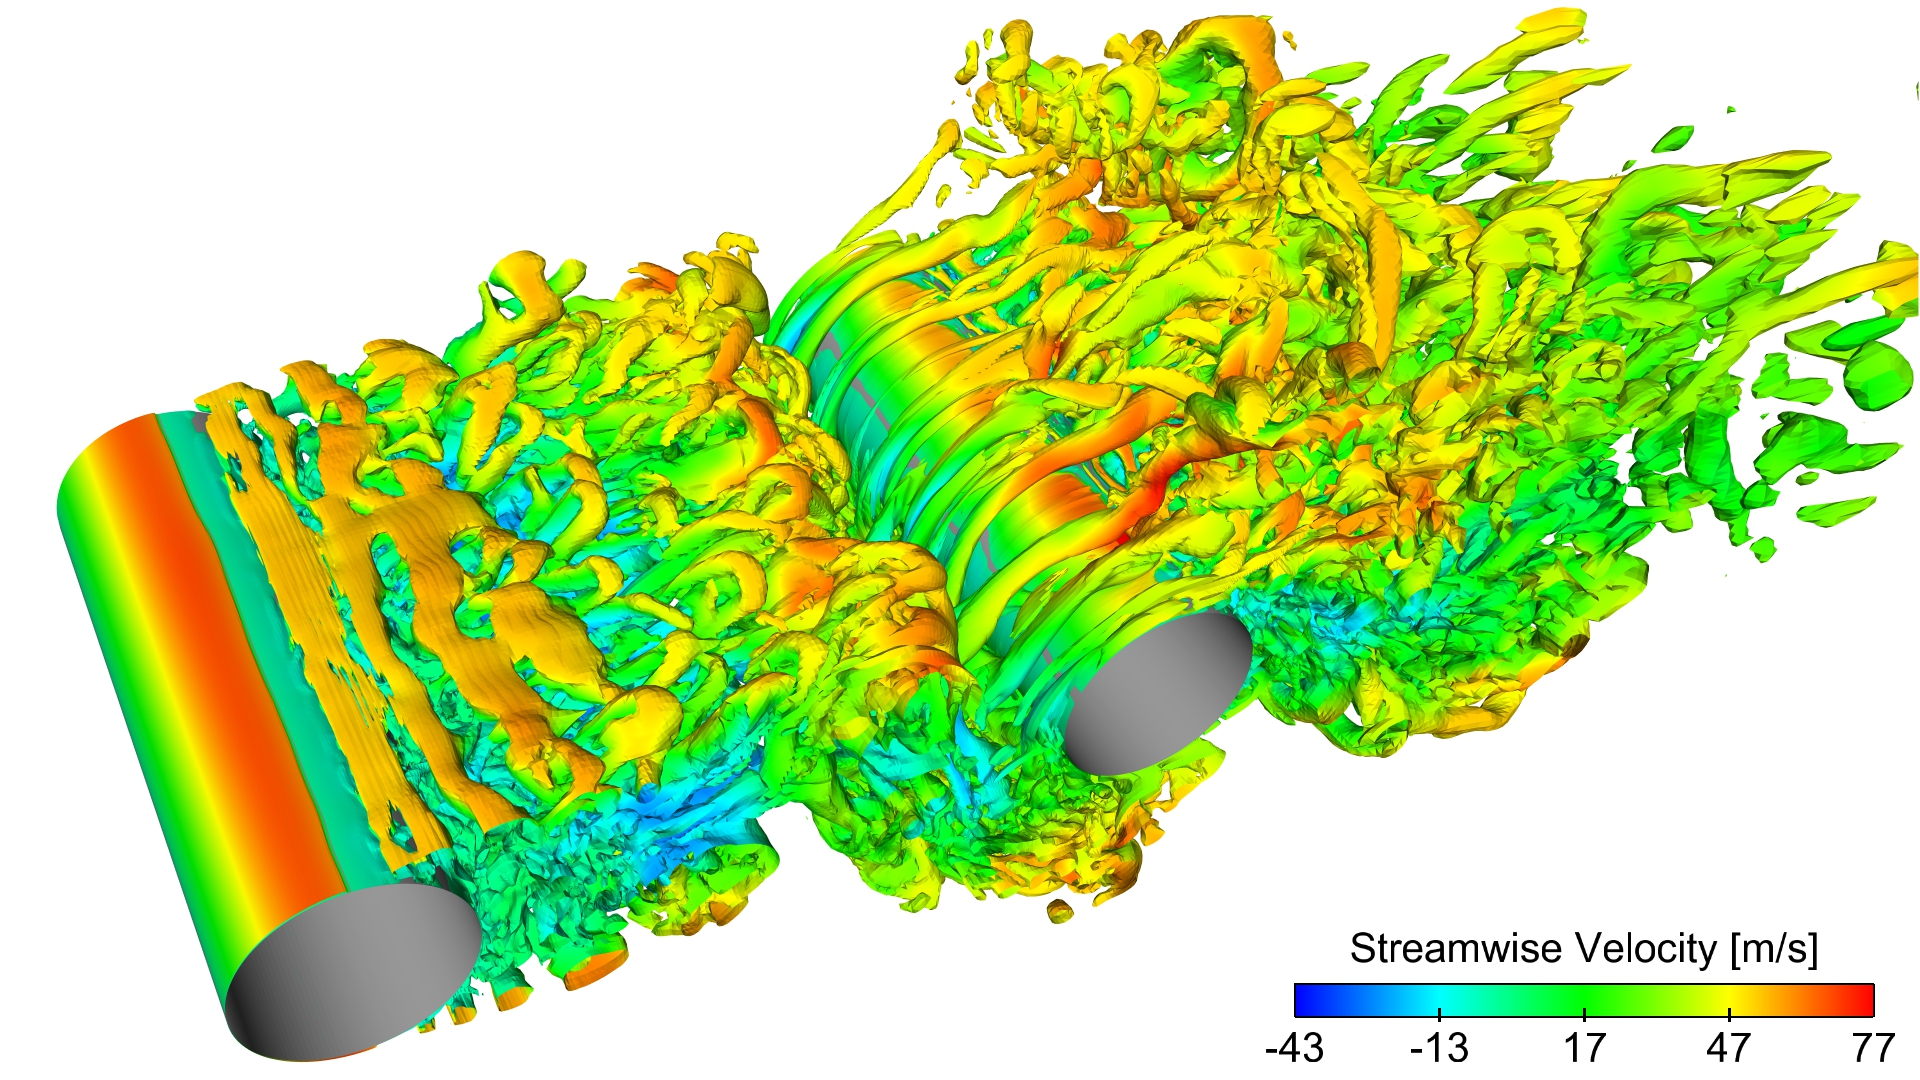
\includegraphics[width=0.40\textwidth]{tc_q_criteria}
    \bicaption{Q判据等值面图。}{Isocontour of Q criteria.}
    \label{fig:tc_q_criteria}
\end{figure}

如果插图的空白区域过大,以图片\verb|shock_cyn|为例,自动裁剪如图\ref{fig:shock_cyn}。
\begin{figure}[!htbp]
    \centering
     \bicaption{激波圆柱作用。}{Shock-cylinder interaction.}
    %trim option's parameter order: left bottom right top
    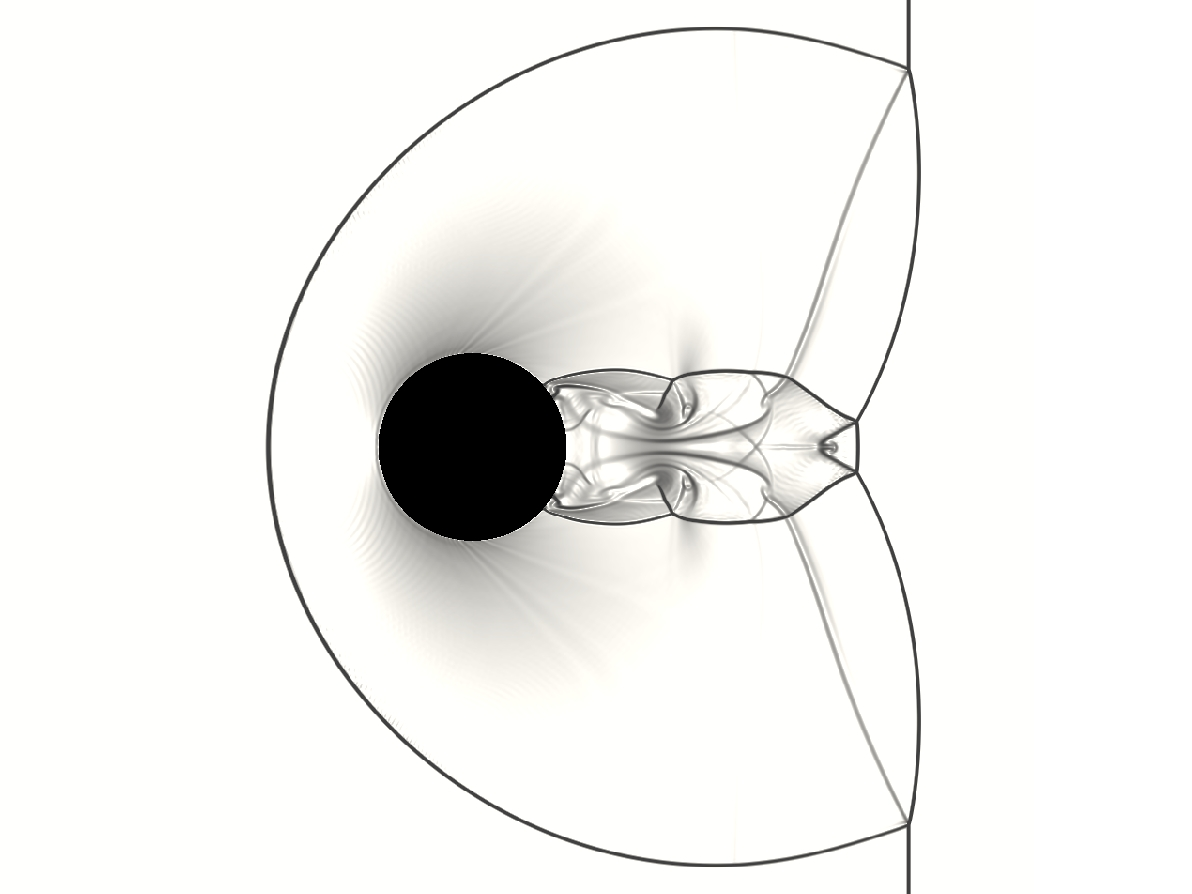
\includegraphics[trim = 30mm 0mm 30mm 0mm, clip, width=0.40\textwidth]{shock_cyn}
   
    \label{fig:shock_cyn}
\end{figure}

多图的插入如图\ref{fig:oaspl}。
\begin{figure}[!htbp]
    \centering
    \begin{subfigure}[b]{0.35\textwidth}
      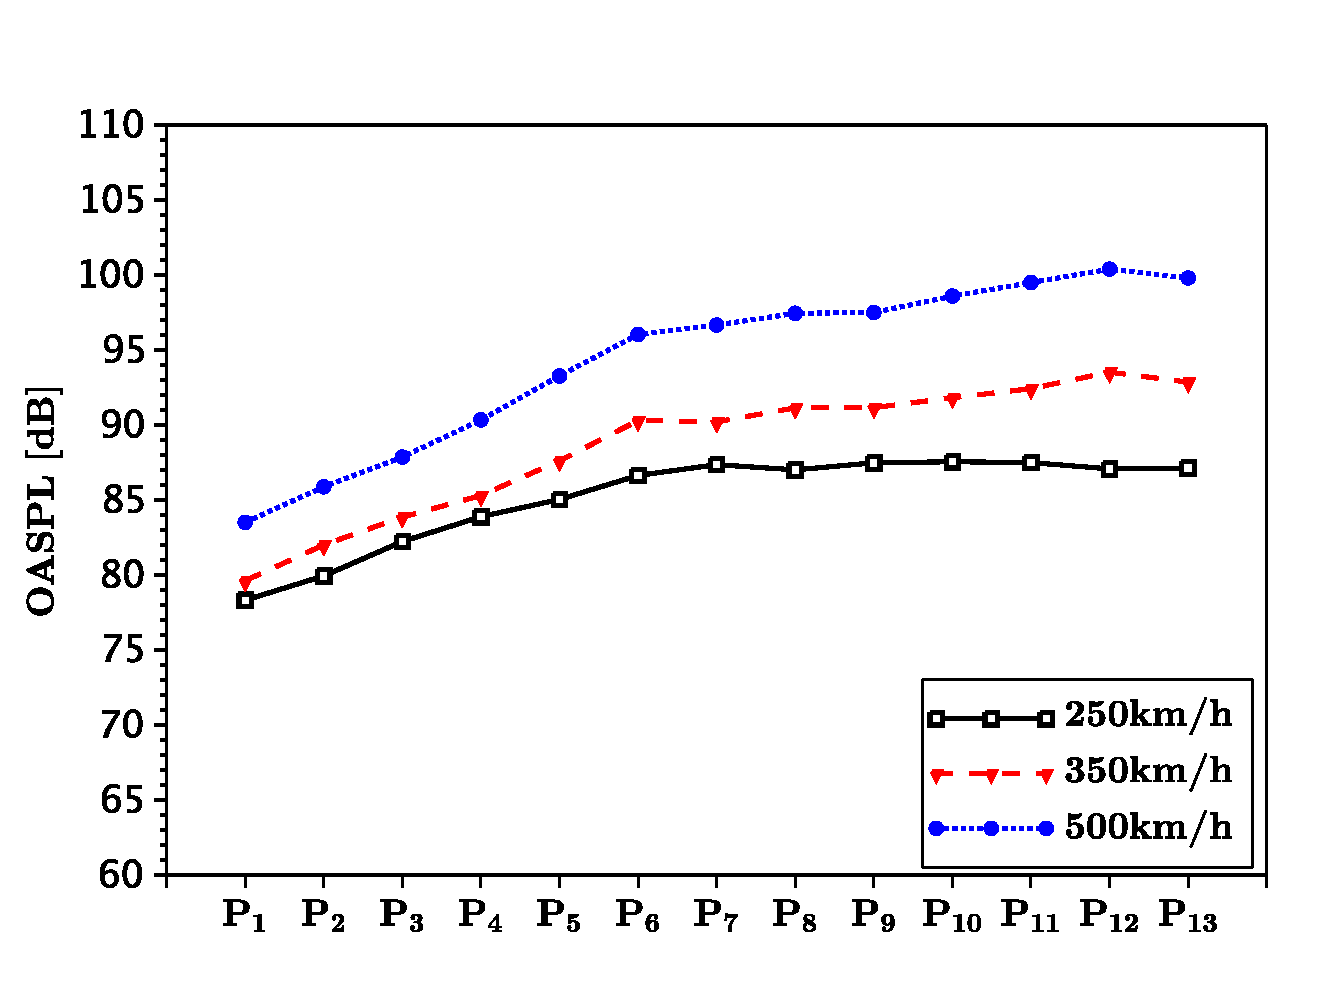
\includegraphics[width=\textwidth]{oaspl_a}
      \caption{}
      \label{fig:oaspl_a}
    \end{subfigure}%
    ~%add desired spacing
    \begin{subfigure}[b]{0.35\textwidth}
      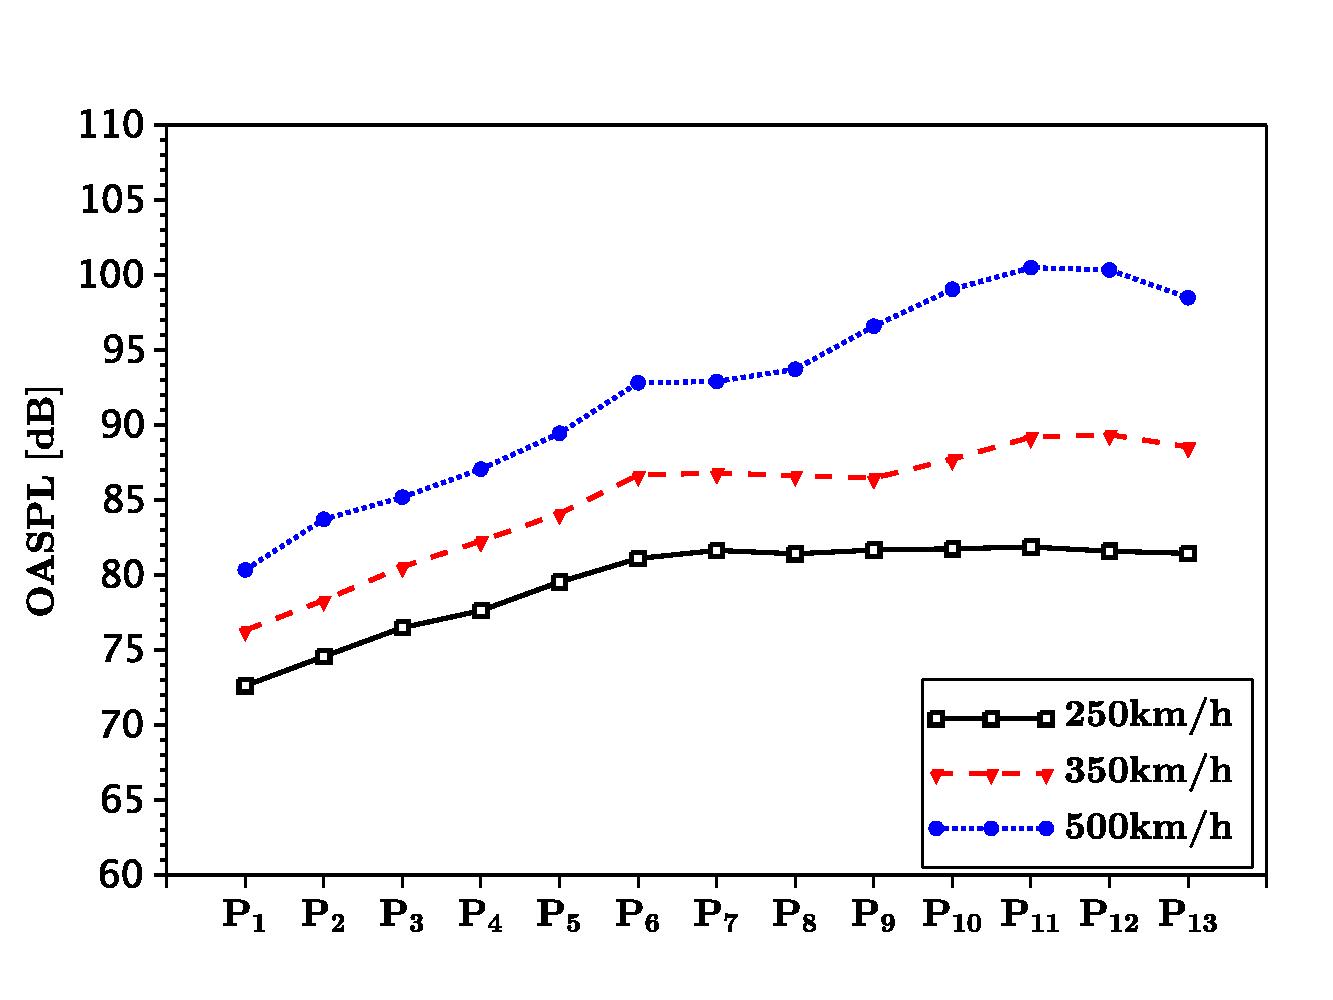
\includegraphics[width=\textwidth]{oaspl_b}
      \caption{}
      \label{fig:oaspl_b}
    \end{subfigure}
    \begin{subfigure}[b]{0.35\textwidth}
      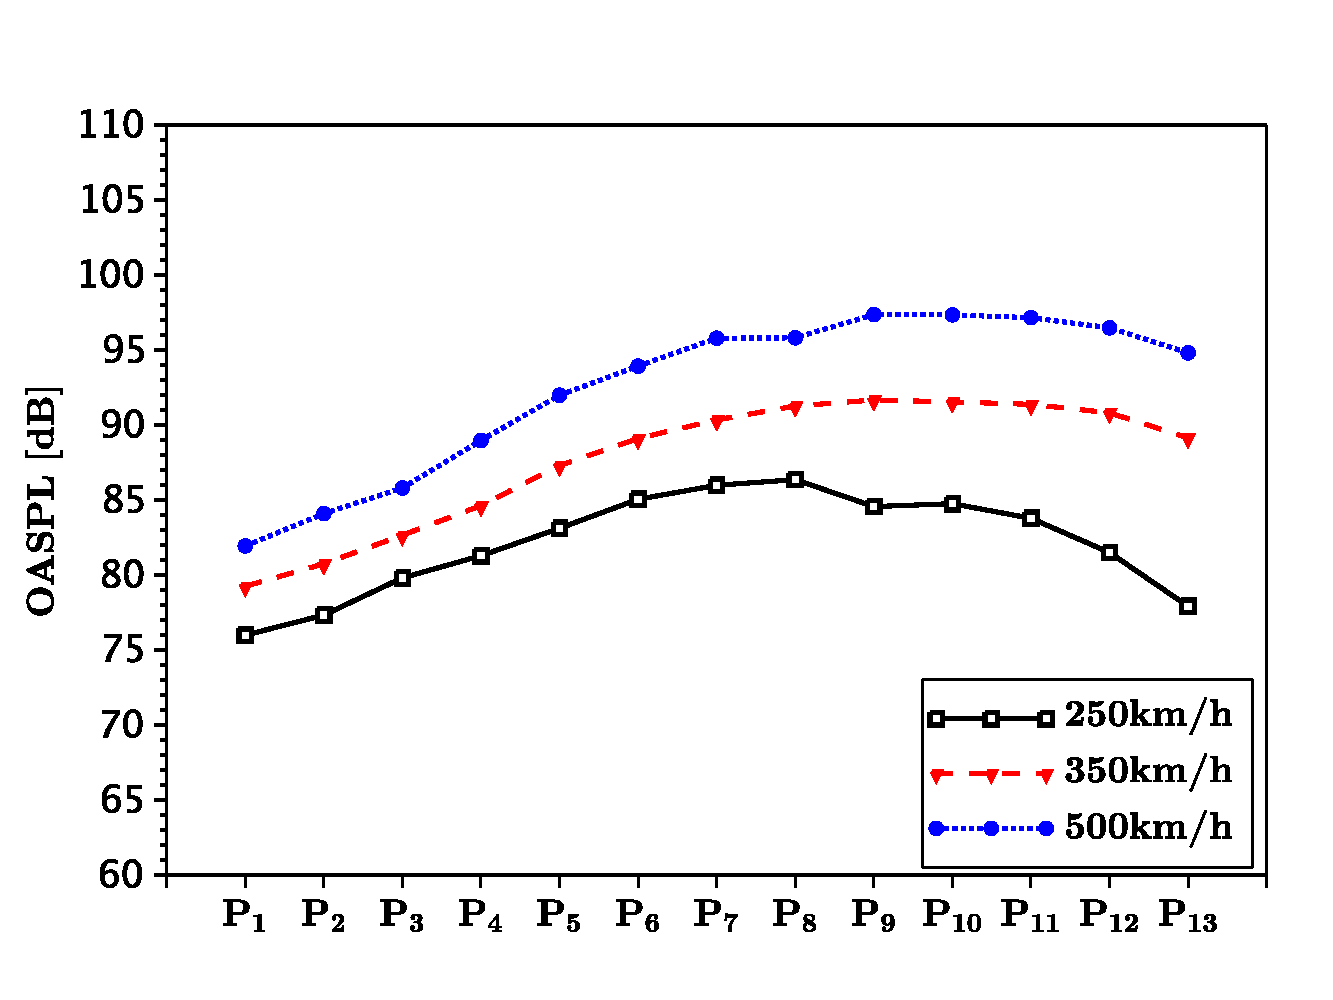
\includegraphics[width=\textwidth]{oaspl_c}
      \caption{}
      \label{fig:oaspl_c}
    \end{subfigure}%
    ~%add desired spacing
    \begin{subfigure}[b]{0.35\textwidth}
      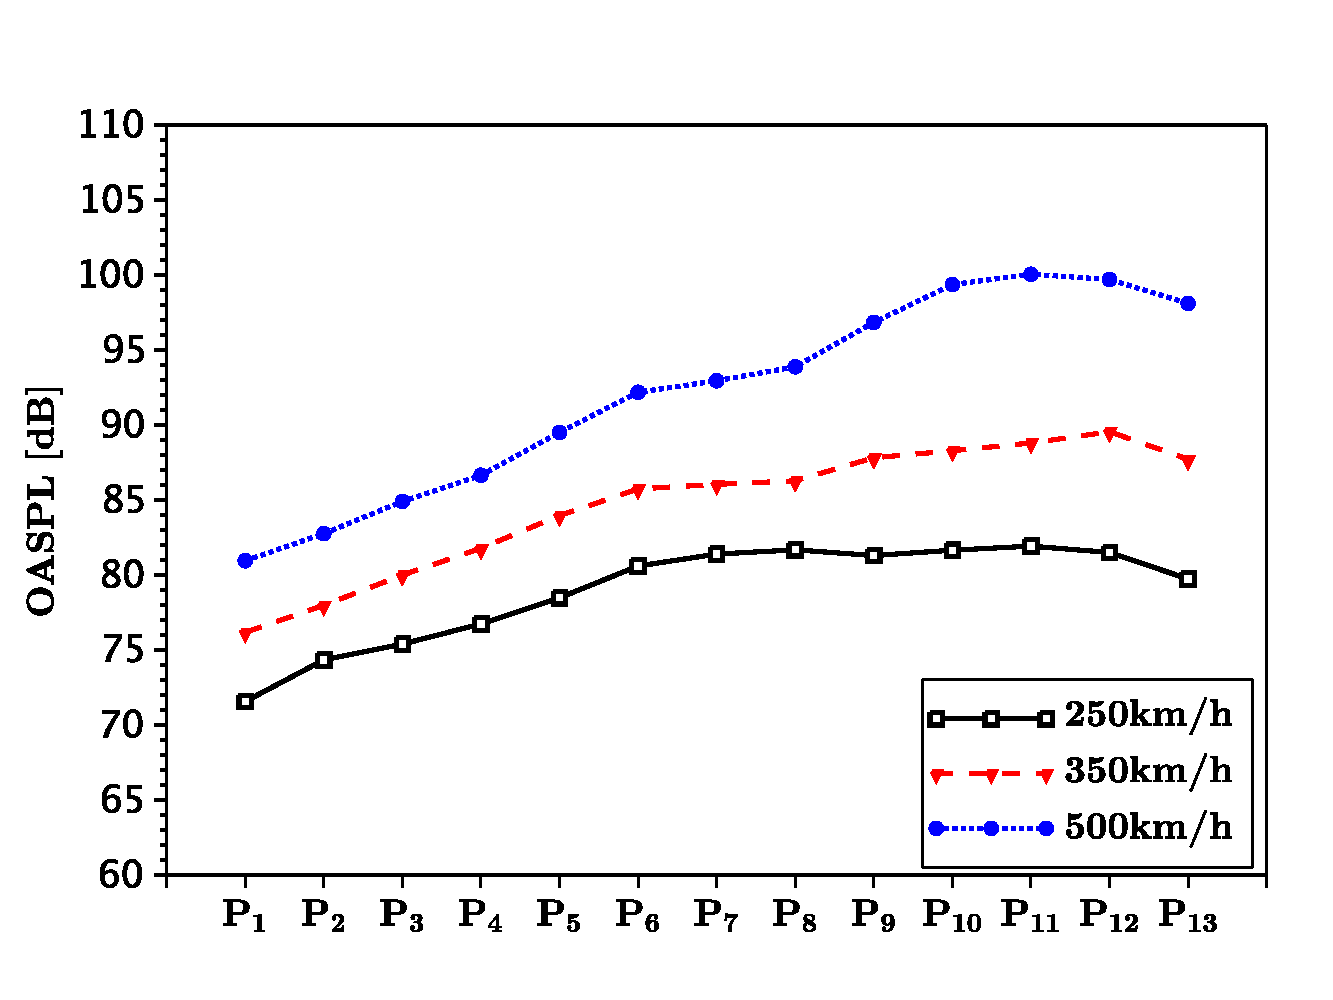
\includegraphics[width=\textwidth]{oaspl_d}
      \caption{}
      \label{fig:oaspl_d}
    \end{subfigure}
    \bicaption{总声压级。(a)$A$,(b)$B$,(c)$C$,(d)$D$。}{OASPL.(a)$A$,(b)$B$,(c)$C$,(d)$D$.}
    \label{fig:oaspl}
\end{figure}

插图的参考代码在\verb|Tex/Commands.tex|亦进行了汇集。

\subsection{算法}

如见算法~\ref{alg:euclid},详细使用方法请参见文档 \href{https://ctan.org/pkg/algorithmicx?lang=en}{algorithmicx}。

\begin{algorithm}[!htbp]
    \small
    \caption{Euclid's algorithm}\label{alg:euclid}
    \begin{algorithmic}[1]
        \Procedure{Euclid}{$a,b$}\Comment{The g.c.d. of a and b}
        \State $r\gets a\bmod b$
        \While{$r\not=0$}\Comment{We have the answer if r is 0}
        \State $a\gets b$
        \State $b\gets r$
        \State $r\gets a\bmod b$
        \EndWhile\label{euclidendwhile}
        \State \textbf{return} $b$\Comment{The gcd is b}
        \EndProcedure
    \end{algorithmic}
\end{algorithm}

\subsection{参考文献引用}

参考文献引用过程以实例进行介绍,假设需要引用名为"Document Preparation System"的文献,步骤如下:

1)使用Google Scholar搜索Document Preparation System,在目标条目下点击Cite,展开后选择Import into BibTeX打开此文章的BibTeX索引信息,将它们copy添加到ref.bib文件中(此文件位于Biblio文件夹下)。

2)你会发现索引信息中第一行为 \verb|@article{lamport1986document,|。其中 \verb|lamport1986document| 即为此文献的label (\textbf{中文文献也必须使用英文label},一般遵照:姓氏拼音+年份+标题第一字拼音的格式),想要在论文中索引此文献,有两种索引类型:

文本类型:\verb|\citet{lamport1986document}|。正如此处所示 \citet{lamport1986document}; 

括号类型:\verb|\citep{lamport1986document}|。正如此处所示 \citep{lamport1986document}。

\textbf{多文献索引用英文逗号隔开}:

\verb|\citep{lamport1986document,chen2005zhulu}|。正如此处所示 \citep{lamport1986document,chen2005zhulu}

如此,即完成了文献的索引,请查看下本文档的参考文献一章,看看是不是就是这么简单呢?是的,就是这么简单!

不同文献样式和引用样式可在Thesis.tex中对artratex.sty调用实现,如:
\begin{itemize}
    \footnotesize
    \item \verb+\usepackage[numbers]{artratex}+ $\%$ 文本: Jones [1]; 括号: [1]
    \item \verb+\usepackage[super]{artratex}+ $\%$ 文本: Jones 上标[1]; 括号: 上标[1]
    \item \verb+\usepackage[authoryear]{artratex}+ $\%$ 文本: Jones (1995); 括号: (Jones, 1995)
    \item \verb+\usepackage[alpha]{artratex}+ $\%$ 文本: 不可用; 括号: [Jon95]
\end{itemize}

%若在上标(super)模式下,希望在特定位置将上标改为嵌入式标,可使用
%
%文本类型:\verb|\citetns{lamport1986document,chen2005zhulu}|。
%
%正如此处所示\citetns{lamport1986document,chen2005zhulu}
%
%括号类型:\verb|\citepns{lamport1986document,chen2005zhulu}|。
%
%正如此处所示\citepns{lamport1986document,chen2005zhulu}

参考文献索引更为详细的信息,请见 \href{https://en.wikibooks.org/wiki/LaTeX/Bibliography_Management}{WiKibook Bibliography}。

\nocite{*}

\section{常见使用问题}\label{sec:qa}

\begin{enumerate}
    \item 模板每次发布前,都已在Windows,Linux,MacOS系统上测试通过。下载模板后,若编译出现错误,则请遵从 \href{https://github.com/mohuangrui/ucasthesis}{位于主页底部的用户指南}。

    \item 模板文档的编码为UTF-8编码。所有文件都必须采用UTF-8编码,否则编译后生成的文档将出现乱码文本。若出现文本编辑器无法打开文档或打开文档乱码的问题,请检查您使用的编辑器对UTF-8编码的支持。如果使用WinEdt作为文本编辑器(不推荐使用),应在其Options -> Preferences -> wrapping选项卡下将两种Wrapping Modes中的内容:
        
        TeX;HTML;ANSI;ASCII|DTX...
        
        修改为:TeX;\textbf{UTF-8|ACP;}HTML;ANSI;ASCII|DTX...
        
        同时,取消Options -> Preferences -> Unicode中的Enable ANSI Format。

    \item 推荐选择xelatex或lualatex编译引擎编译中文文档。编译脚本的默认设定为xelatex编译引擎。你也可以选择不使用脚本编译,如直接使用 \TeX{}文本编辑器编译。注:\TeX{}文本编辑器编译的默认设定为pdflatex编译引擎,若选择xelatex或lualatex编译引擎,请进入下拉菜单选择。为正确生成引用链接,需要进行全编译。
    \item Texmaker使用简介
        \begin{enumerate}
            \footnotesize
            \item 使用 Texmaker “打开” Thesis.tex。
            \item 菜单 “选项 (Options)” -> “设置当前文档为主文档 (Define as Master Document)”
            \item 菜单 “自定义 (User)” -> “自定义命令 (User Commands)” -> “编辑自定义命令 (Edit User Commands)” -> 左侧选择 “command 1”,右侧 “菜单项 (Menu Item)” 填入 Auto Build -> 点击下方“向导 (Wizard)” -> “添加 (Add)”: xelatex + bibtex + xelatex + xelatex + pdf viewer -> 点击“完成 (OK)”
            \item 使用 Auto Build 编译带有未生成引用链接的源文件,可以仅使用 xelatex 编译带有已经正确生成引用链接的源文件。
            \item 编译完成,“查看(View)” PDF,在pdf中 “ctrl+click” 可链接到相对应的源文件。
        \end{enumerate}
    
    \item 模版的设计可能地考虑了适应性。致谢等所有条目都是通过最为通用的

        \verb+\chapter{item name}+  and \verb+\section*{item name}+

        来显式实现的 (请观察Backmatter.tex),从而可以随意添加,放置,和修改,如同一般章节。对于图表目录名称则可在ucasthesis.cfg中进行修改。

    \item 设置文档样式: 在artratex.sty中搜索关键字定位相应命令,然后修改
        \begin{enumerate}
            \item 正文行距:启用和设置 \verb|\linespread{1.5}|,默认1.5倍行距。
            \item 参考文献行距:修改 \verb|\setlength{\bibsep}{0.0ex}|
            \item 目录显示subsection:修改 \verb|\setcounter{tocdepth}{2}|
            \item 文档内超链接的颜色及其显示:修改 \verb|\hypersetup|
            \item 页眉页脚的设定:frontmatterstyle,mainmatterstyle,和backmatterstyle分别用于定义前言,主要内容,和附录的页眉页脚样式。通过阅读这一部分的代码,可以轻松地理解和修改以获得自定义的样式。命令的详细解释请参见 \href{https://www.ctan.org/pkg/fancyhdr?lang=en}{fancyhdr} 的用户文档。同时可参见 \href{https://ctan.org/pkg/ctex?lang=en}{ctex} 宏包用户文档。

            \item 设置图2.3为图2-3: 设置
                {
                    \footnotesize
\begin{verbatim}
\renewcommand{\theequation}{\arabic{chapter}-\arabic{equation}}
\renewcommand{\thefigure}{\arabic{chapter}-\arabic{figure}}
\renewcommand{\thetable}{\arabic{chapter}-\arabic{table}}
\end{verbatim}
                }
        \end{enumerate}

    \item 字体控制。文档内字体切换方法:
        \begin{itemize}
            \item 宋体:飞扬跋扈~或 \textrm{飞扬跋扈}
            \item 粗宋体:{\bfseries 飞扬跋扈} 或 \textbf{飞扬跋扈}
            \item 黑体:{\sffamily 飞扬跋扈} 或 \textsf{飞扬跋扈}
            \item 粗黑体:{\bfseries\sffamily 飞扬跋扈} 或 \textsf{\bfseries 飞扬跋扈}
            \item 仿宋:{\ttfamily 飞扬跋扈} 或 \texttt{飞扬跋扈}
            \item 楷体:{\itshape 飞扬跋扈} 或 \textit{飞扬跋扈}
        \end{itemize}
        
        由于缺乏一个统一的被各个操作系统所默认携带的完备的中文字体库,\href{https://ctan.org/pkg/ctex?lang=en}{ctex} 针对不同的操作系统而调用各系统上所对应的一类中文字体库。由于很多操作系统的字库往往缺乏原生态的加粗宋体字重,有时会发生加粗宋体被黑体所替换的情形,这对封面的字体造成影响。若需要解决这个问题,可采用调用自定义的一个完备字体库的方案。
        
        若需设置字体库,请选择xelatex或lualatex编译引擎,并设置需要的字体库。如用Times New Roman作为英文字体,在artratex.sty中设置:

                 \verb|\setmainfont{Times New Roman}|

                 如果需要调用一个自定义的中文字体库,方法为:

                \begin{itemize}
                    \item 调用 \href{https://ctan.org/pkg/ctex?lang=en}{ctex} 预定义好的备用字库: 在Thesis.tex中设置

                        {
                            \small
                            \verb|\documentclass[doublesided,fontset=fandol]{Style/ucasthesis}%|
                         }

                         便可调用 \href{https://ctan.org/tex-archive/fonts/fandol?lang=en}{fandol} 这一字体库。\LaTeX{}编译系统一般已携带或是能自动下载安装 \href{https://ctan.org/tex-archive/fonts/fandol?lang=en}{fandol} 字库。若不能,则请手动下载并安装链接所提供的所有字体即可。本模板使用说明文档就是采用调用 \href{https://ctan.org/tex-archive/fonts/fandol?lang=en}{fandol} 中文字库。

                     \item 手动调用系统带有的中文字库: 首先需要查看系统所带有的中文字库及其名称,也可选择安装可获得的中文字库。假设系统已安装或带有名为SC的中文字库(此字库为MacOS所配备,具备原生态的加粗宋体),则可在artratex.sty的

                         \verb|\RequirePackage{fontspec}|

                        行下添加如下中文字体调用命令:
                        {
                            \scriptsize
\begin{verbatim}
\setCJKmainfont[BoldFont=Songti SC Bold,ItalicFont=Kaiti SC]{Songti SC Light}%
\setCJKsansfont{Heiti SC}%
\end{verbatim}
                        }
                \end{itemize}

                字库调用的全面解释可参见 \href{https://ctan.org/pkg/fontspec}{fontspec} (英文字体调用)和 \href{https://ctan.org/pkg/xecjk?lang=en}{xeCJK} (中文字体调用)。因为模版的设定考虑兼顾不同操作系统(Windows, Linux, Mac OS),为了模版的健壮性,上述字体设置和调用方案并未作为原始设定。
            \item 封面下划线上的文本不居中下划线,这是因为那些下划线前面还有字头,导致文本只能在页面居中和在下划线上居中二选一。当前封面采取页面居中。如需要调整文本在下划线上的位置,可用 \verb|\hspace{+/- n.0em}| 命令来插入或删除 n 个空格,进行手动调整,比如

                \verb|\advisor{\hspace{+3.0em} xxx~研究员~xxx单位}|
                
                这个解决方案是很不优雅,但问题本质还是样式的设计问题。有时下划线看上去粗细不一致,这是显示的问题,打印正常。
    \item  一般规范下,章应开始于奇数页。从而若前一章结束于奇数页,则一空白页将被插入以保证上述规则。如想修改以取消空白页,有如下方案:
     \begin{itemize}
         \item 在thesis.tex的documentclass中用singlesided替代doublesided。这使文档不区分奇偶页,因此章可以开始于任意页。此方案将移除所有空白页,包括封面处的。同时,页眉页脚的设定不再区分奇偶页。
         \item 可以在ucasthesis.cls文件中,将cleardoublepage命令的定义修改为:

             \verb|\def\cleardoublepage{\clearpage}|

             这一命令使产生空白页的机制失效。这一方案将移除所有的空白页,包括封面处的。但与方案一不同的是,页面页脚的设定可以区分奇偶页。
         \item 在thesis.tex的documentclass中添加openany选项(openany与doublesided和printcopy都可搭配)。这一命令使章可以开始于任意页。同时,将artratex.sty中和thesis.tex中的cleardoublepage改为clearpage。此方案将移除所有的用于调整章的起始位置的空白页,而不包括封面处的。同时,页面页脚的设定可以区分奇偶页。
     \end{itemize}
      无论哪种方案都要注意对页眉页脚的影响并做出合适的调整。推荐是采用默认设置,尽量避免将精力花在这些无关紧要的细节上。\LaTeX{}的特点是标准化,而其导致的问题则是任何脱离标准的修改都将花费相当精力。对于电子档的论文,在thesis.tex的documentclass中,若不想使用doublesided,则可使用singlesided来减少空白页。而对于打印版,启用printcopy选项以替换doublesided/singlesided选项,这样可使奇偶页的排版在打印装订后更美观。

  \item 部分所也许对格式有不同设定,因\LaTeX{}将内容与格式分离,格式的调整可独立于内容进行,并只需修改模板样式文件完成,并无风险。
\end{enumerate}



%%% ++++++++++++++++++++++++++++++++++++++++++++++++++++++++++++++++++++++++++++++++++
%
%%%%% --------------------------------------------------------------------------------
%%
%%%%******************************** Appendix ****************************************
%%
%% Some subordinate chapters.
\cleardoublepage
\appendix%

\chapter[附\quad 录]{附录\quad 中国科学院大学学位论文撰写要求}

学位论文是研究生科研工作成果的集中体现,是评判学位申请者学术水平、授予其学位的主要依据,是科研领域重要的文献资料。根据《科学技术报告、学位论文和学术论文的编写格式》(GB/T 7713-1987)、《学位论文编写规则》(GB/T 7713.1-2006)和《文后参考文献著录规则》(GB7714—87)等国家有关标准,结合中国科学院大学(以下简称“国科大”)的实际情况,特制订本规定。
%
%%%%% --------------------------------------------------------------------------------
%%
%%%%******************************* Backmatter ***************************************
%%
%% Matters of Bibliography, Glossary, Index.
\backmatter
%%
%%% >>> Bibliography
%%
\intotoc{\bibname}% add a corresponding item to the contents table and bookmark
\bibliography{Biblio/ref}%
%%
%%% >>> Other contents
%%
\chapter{致\quad 谢}

值此论文完成之际,谨在此向多年来给予我关心和帮助的老师、学长、同学、
朋友和家人表示衷心的感谢!

没有~ctex package~的众多前辈的辛勤付出和~CASthesis package~作者吴凌云学长的贡献,
~\LaTeX{}~菜鸟的我是无法完成此学位论文模板的。在~\LaTeX{}~中的一点一滴的成长源于
开源社区的众多资料和教程,在此对所有前辈们的付出表示感谢!

......

谨把本文献给我最敬爱的父亲!


\rightline{张三}
\rightline{2018年6月}


\chapter{作者简历及攻读学位期间发表的学术论文与研究成果}

\section*{作者简历}

\subsection*{casthesis作者}

吴凌云,男,福建省屏南县人,1975 年出生,中国科学院数学与系统科学研究院博士研究生。

通讯地址:北京市~2734 信箱,中科院数学与系统科学研究院应用数学所

邮编:100080

E-mail: aloft@ctex.org

\subsection*{ucasthesis作者}

莫晃锐,男,湖南省湘潭县人,1989 年出生,中国科学院力学研究所硕士研究生。

通讯地址:北京市北四环西路15号中国科学院力学研究所

邮编:100190

E-mail: mohuangrui@gmail.com

\begin{description}
 \item[获奖情况:] XXX
 \item[\quad\quad\quad\quad\quad] XXX
 \item[\quad\quad\quad\quad\quad] XXX
\end{description}


\section*{已发表(或正式接受)的学术论文:}

\noindent
一作论文:
\setcounter{mycnt}{0}

\noindent
\stepaddpaper \hangindent=0.7cm\hangafter=1 Stamerjohanns H, Ginev D, David C, et al. MathML-aware article conversion from LaTeX [J]. Towards a Digital Mathematics Library, 2009, 16(2): 109–120.

\noindent
\stepaddpaper \hangindent=0.7cm\hangafter=1 Thesis Template of the University of Chinese Academy of Sciences, 2014.


\noindent
合作论文:
\setcounter{mycnt}{0}
\newline\noindent
\stepaddpaper 作者发表的论文.
\newline\noindent
\stepaddpaper 作者发表的论文.
\newline\noindent
\stepaddpaper XXXX.


\section*{申请或已获得的专利:}

(无专利时此项不必列出)

\section*{参加的研究项目及获奖情况:}

可以随意添加新的条目或是结构




%%
\end{document}
%%%%% --------------------------------------------------------------------------------
